
After calibrating the time of flight parameter, we can start calibrating the readout pulse through resonator characterization.\\
The first thing to do is to find the resonator frequency, that is to say its transition frequency.

At this frequency we will be able to observe a clear difference in the transmitted signal: if the resonator is a 3D cavity we will observe an amplified signal, while for a 2D resonator we will observe a higher absorption.
In both cases, we expect to see a Lorentzian peak (positive for 3D cavity or negative for 2D resonators):
\begin{equation}
    y=y_0 + \frac{w^2}{4(x-x_0)^2+w^2}
\end{equation}
Where $w$ is equal to half of the peak width.

In the experiment, we send a readout pulse with fixed duration and amplitude and, after waiting for the TOF, we acquire a waveform that we average, obtaining a single point. 
We then repeat the experiment for different frequencies, ideally obtaining a plot like the one sketched in \cref{fig:resonator_spectroscopy_sketch}.

\begin{figure}[ht]
    \centering
    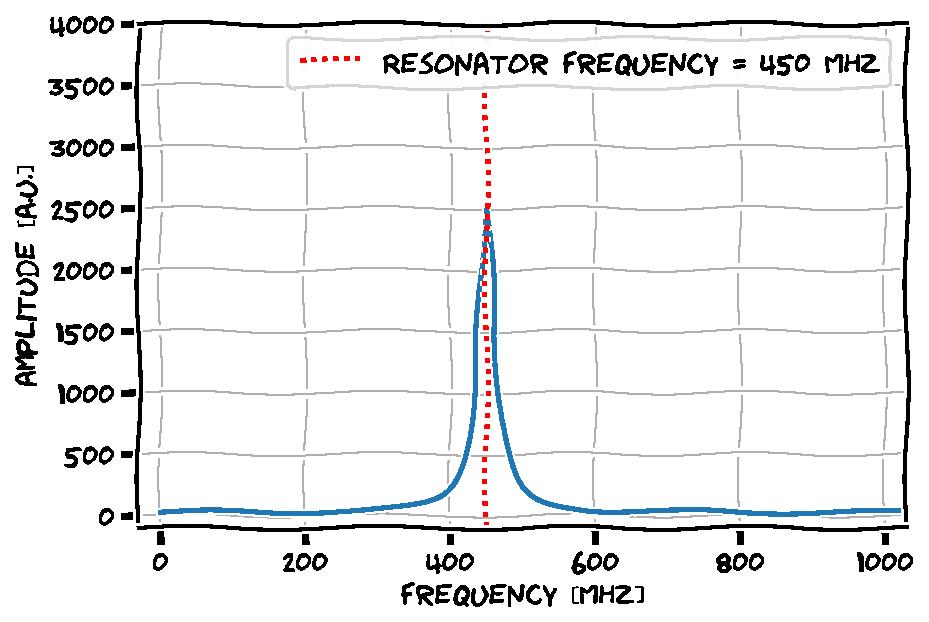
\includegraphics[width=8cm]{characterization/figures/resonator_spectroscopy_sketch.pdf}
    \caption{Plot of a generic resonator spectroscopy experiment.}
    \label{fig:resonator_spectroscopy_sketch}
\end{figure}

In the time of flight experiment we didn't really have many variables, for the resonator spectroscopy, on the other hand, the situation is very different.
In particular, we are extremely dependent on the amplitude of the pulse and on its duration\footnote{Note that, for the readout pulse we usually use a rectangular waveform. For the control pulse, the shape is a much more relevant parameter, that will require a specific calibration.}.
Since the objective of this experiment is to find the resonator frequency, without any readout optimization (something that we will have to do afterwards), we can fix the duration of the pulse at $2\,\mu$s.

For the amplitude the discussion is slightly more complex and there are several elements to take into consideration:
\begin{itemize}
    \item higher amplitudes usually correspond to better S/N;
    \item at high amplitudes the signal breaks superconductivity, therefore resonator is not effectively not coupled to the qubit (we talk of \textbf{bare resonator frequency});
    \item at intermediate amplitudes the peak could completely disappear and is, in general, not Lorentzian;
    \item very high amplitudes could damage the components\footnote{This is especially true in the case of a 3D cavity, where the delicate qubit is inside the cavity and the line is shared both by control and readout.}.
\end{itemize}

In the first stages of characterization, we do not need to be at low power to operate: even if the resonator is not coupled to the qubit it is not a problem\footnote{By "not coupled with the qubit" we mean that, since we send a huge number of photons through our readout line, we are essentially exceeding the Josephson junction critical current and "turning off" the qubit.}.
Indeed it is preferable to have higher S/N so that the peak is clearly identifiable.
With standard attenuation inside the fridge ($-55$ dB + line resistance), a reasonable voltage could be around $0.5$ V. 
However, different instruments have different way of controlling the power: some may offer attenuation control, some just a linear amplification. 
The experimenter will, inevitably, have to decide power levels dependently from its setup.

Another parameter connected to the amplitude, is also the \textit{relaxation time} (in some literature also referred to as \textit{repetition duration}) and the number of shots.
The number of shots represents the number of repetitions of the same experiment (at the same frequency), while the relaxation time is the waiting time between repetitions.
A higher number of shots will increase the S/N ratio by averaging the noise, but will also slow down the acquisition.
As per the relaxation time, for this experiment in particular we can leave it at zero: since we are not exciting the qubit we do not particularly care about it. 
However note that, for 3D cavities, we could end up damaging the qubit if we send too much energy over a small period of time so it could be worth to increase the relaxation time.

Last but not least, we have to choose which frequencies are probed during the scan: a very wide scan can be useful if nothing is known about the studied resonator, but in general we have at least the design parameters.
These are often not exact, but can give an idea of the region to scan (for standard cavities around $7$ GHz).
Also, a very small step between two subsequent frequency points is not needed and could really slow down the experiment (from seconds to tens of minutes) if chosen incorrectly.
Usually, a step of $200$ MHz is fine enough.

A plot for a resonator spectroscopy experiment is presented \cref{fig:resonator_spectroscopy_3D}.
This plot was obtained probing a 3D cavity resonator with a \RFSoC board that, since can synthesize frequency up to $9.8$ GHz, didn't require any external local oscillator for the upconversion.

\begin{figure}[ht]
    \makebox[\textwidth][c]{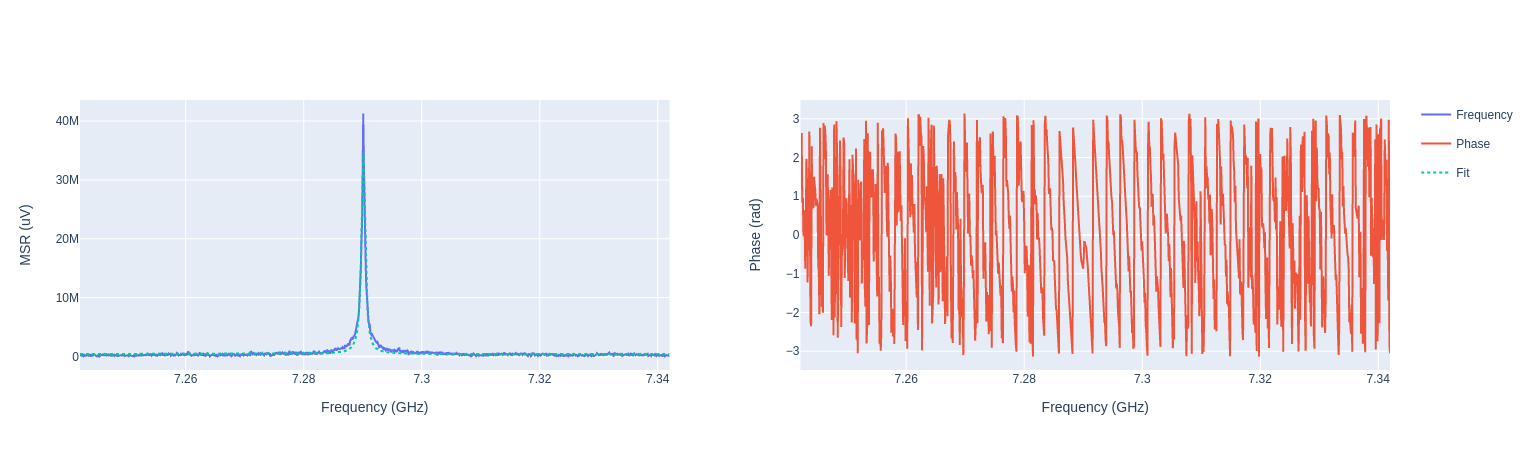
\includegraphics[width=1.3\textwidth]{characterization/figures/resonator_spectroscopy_3D.png}}
    \caption{Resonator spectroscopy, for a 3D cavity.}
    \label{fig:resonator_spectroscopy_3D}
\end{figure}

The use of a 3D resonator is a special case that generally leads to better S/N, as well as less overall noise and a horizontal background, in respect to planar chips.\\
For example, in \cref{fig:resonator_spectroscopy_2D}, we can see a resonator spectroscopy done on a chip namely containing 5 different multiplexed\footnote{By multiplexed we mean that the resonator are coupled to the same readout line and can be probed simultaneously.} resonators (was not possible to identify one of them).\\
The experiment was conducted with a \ZCU board, with a firmware that enables multiplexed readout (so the use of a common DAC and ADC for the simultaneous readout of multiple resonators), with the drawback of a limited bandwidth. 
Because of that, a local oscillator is needed along with an IQ mixer.
Unfortunately, this configuration carries some problem, most notably:
\begin{itemize}
    \item the background is noisier and less horizontal;
    \item the upconversion scheme creates multiple "images" of the upconverted signals;
    \item background-resonance interaction can severely change the shape of the peak (from a Lorentzian to a Fano resonance~\cite{Fano1961, Limonov2017});
    \item the frequency value of the local oscillator has a strong effect on the overall background.
\end{itemize}

All of these phenomena can be seen in \cref{fig:resonator_spectroscopy_2D} (resonator 4, for example, is a Fano resonance, while resonator 3 isn't).

\begin{figure}[ht]
    \centering
    \makebox[\textwidth][c]{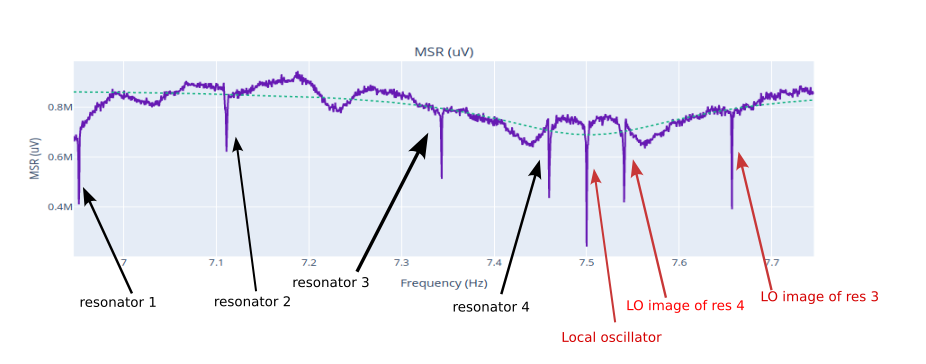
\includegraphics[width=1.3\textwidth]{characterization/figures/resonators.png}}
    \caption{Resonator spectroscopy, for multiple multiplexed 2D resonators with a local oscillator for upconversion.}
    \label{fig:resonator_spectroscopy_2D}
\end{figure}

Common problems that could increase the difficulty of this experiment generally involve the power level (amplitude) set for the pulse, that could be too low to clearly see the peak, or the use of very large frequency step that could reduce the number of samples actually part of the resonance.\\
Note that this experiment does not really require the use of a FPGA or a RFSoC and can be initially performed with a VNA (generally easier/faster to use). 
However, being able to perform all the experiments without needing to change the hardware setup can be extremely beneficial. 

Focusing on a single peak, both for the 3D and the 2D case, at this point we should have roughly found the resonant frequency: that is the main objective of this experiment.
Although it is not strictly required, we can fit the peak with a Lorentzian/Fano resonance on a background, to extract the frequency with more precision and to compute the resonator quality factor \textit{in the high power regime} that can be defined equivalently as:
\begin{equation}
    Q=\frac{f_r}{\Delta f_r}= \frac{\omega_r}{\Delta \omega_r} = 2\pi f_r\frac{\text{energy store}}{\text{power loss}}
\end{equation}
Where $f_r$ is the resonator frequency, $\Delta f_r$ the peak width and $2\pi f = \omega$.

These information are not strictly required for qubit calibration, but could help to understand the overall quality of the system.

\experimentrecap
{Resonator spectroscopy (high power regime)}
{readout calibration}
{bare resonator frequency,\\resonator quality factor (in high power)}
{a measurement (readout pulse fired, averaged acquisition after TOF) is executed for different frequencies. We plot acquired amplitude Vs frequency, we look for a Lorentzian peak (or Fano resonance) and extract the bare resonator frequency as the minimum (2D resonators) or maximum (3D cavity)}
